% article example for classicthesis.sty
\documentclass[10pt,a4paper]{article} % KOMA-Script article scrartcl
\usepackage{lipsum}
\usepackage{url}
\usepackage{amsmath}
\usepackage{makecell}
\usepackage[nochapters]{classicthesis} % nochapters
\usepackage{graphicx}
\graphicspath{ {Figures/} }   

\tolerance=1
\emergencystretch=\maxdimen
\hyphenpenalty=10000
\hbadness=10000

\setlength{\parskip}{1em}
 
\begin{document}
    \title{\rmfamily\normalfont{Modifications made in Ranking Formulae}}
    \author{\spacedlowsmallcaps{Vaibhav Kasturia}}
    \date{\vspace{-5ex}}
    
    \maketitle
    
    \section{Relativeness}
    
    A document should be considered more important than another document if query entities in the document
    are more at the beginning of the document compared to the other document.
    We consider the position of entities in the documents and modify the relativeness 
    score of the documents (for {\tt AND} and {\tt OR} semantics) as follows: 
    
    \begin{equation}
    \label{frml:relative_and_exponential}
    score^{f}_{\wedge}(d, E_Q) = \frac{ \sum_{pos(e,d)}{\exp(-a \cdot pos(e,d))}}{\sum_{pos(e',d)}{\exp(-a \cdot pos(e',d))}} \qquad e\in E_Q, e'\in ents(d)
    \end{equation}

    \begin{equation}
    \label{frml:relative_or_exponential}
    score^{f}_{\vee}(d, E_Q) = \frac{ \sum_{pos(e,d)}{\exp(-a \cdot pos(e,d))}}{ \sum_{pos(e',d)}{\exp(-a \cdot pos(e,d))}} \cdot \frac{|ents(d) \cap E_Q|}{|E_Q|} \qquad e\in E_Q, e'\in ents(d)
    \end{equation}

    \noindent In \ref{frml:relative_and_exponential} and \ref{frml:relative_or_exponential}, $a$ denotes the rate factor of the negative 
    exponential function, $pos(e,d)$ denotes position of entity $e$ in document $d$. 
    The user attention tends to decrease rapidly as he moves across the document. 
    For example, a historian looking for an important document related to an entity may not read the complete document if he doesn't find the entity and the content he is looking for at the beginning. 
    For this reason, we modelled the importance as negative exponential 
    function.
    We also model relativeness score as a linearly decreasing function with position as shown in \ref{frml:relative_and_Linear} and \ref{frml:relative_or_Linear}.  
    
    \begin{equation}
    \label{frml:relative_and_Linear}
    score^{f}_{\wedge}(d, E_Q) = \frac{\sum_{pos(e,d)}{(1-\frac{pos(e,d)}{maxpos(d)})}}{\sum_{pos(e',d)}{(1-\frac{pos(e,d)}{maxpos(d)})}} \qquad e\in E_Q, e'\in ents(d)
    \end{equation}
    
    \begin{equation}
    \label{frml:relative_or_Linear}
    score^{f}_{\wedge}(d, E_Q) = \frac{\sum_{pos(e,d)}{(1-\frac{pos(e,d)}{maxpos(d)})}}{\sum_{pos(e',d)}{(1-\frac{pos(e,d)}{maxpos(d)})}} \cdot \frac{|ents(d) \cap E_Q|}{|E_Q|} \qquad e\in E_Q, e'\in ents(d)
    \end{equation}
    
    \noindent In \ref{frml:relative_and_Linear} and \ref{frml:relative_or_Linear}, $maxpos(d)$ denotes the farthest position of occurrence of an entity in a document $d$. 
    Sum of the negative exponential function for all positions of the query entities and related entities is performed
    keeping the rate factor values as $10^{-3}$, $5 \times 10^{-4}$ and $10^{-5}$. 
    The smaller we keep the decay factor, the slower will be the exponential decay. 
    
    \section{Relatedness}
    
    When we define the relatedness score of a document, we should also keep in mind the difference in position 
    between the query entities and the related entities. We define a measure called {\em proximity} score for 
    each related entity which is based on the position difference of the related entity to the query entity.
    
    \noindent Consider a document in which the red lines denote the positions of a query entity and 
    blue lines denote the positions of a related entity along the length of the document
    as shown in Figure.
    
    \begin{figure}[ht]
	\centering
	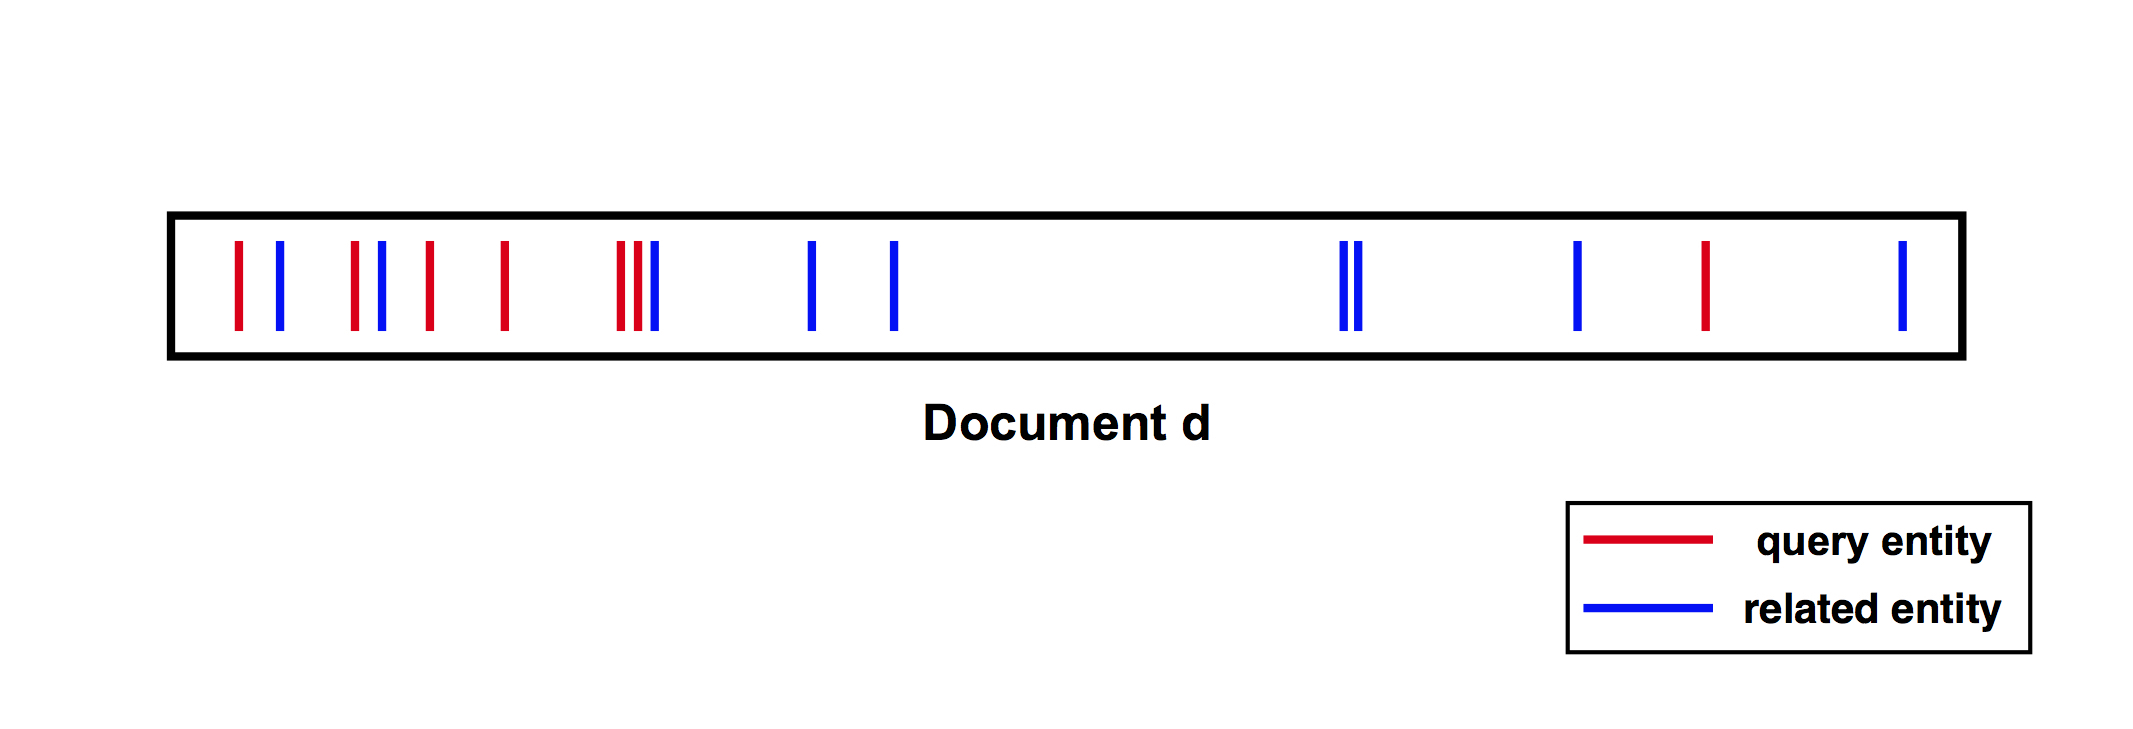
\includegraphics[width=0.95\textwidth]{entity_positions_in_doc.jpg}
	\caption{Positions of a query entity and a related entity inside a document d visualized across its length.}
	\label{fig:entity_positions_in_doc}
    \end{figure}

    \noindent Define $Dist(e,e')$ and $avgDist(e,e')$ as the average distance of a related entity $e$ w.r.t a query entity $e'$ in a document $d$. 
    
    \noindent For the first approach, the average distance is calculated by checking each red line(position of the query entity) 
    in the document. If the red line that we are currently at, is preceded by a blue line and succeeded by a red line (or no line), or preceded by a another red line (or no line) and succeeded by a blue line, then we take $Dist(e,e')$ as the the absolute difference in position between current red line and the blue line. 
    However, if the red line that we are currently at is preceded and succeeded by blue lines, then we take $Dist(e,e')$ as the average of the absolute difference in position between the current red line and the each blue line.
    Also, if we are currently at a red line which is preceded and succeeded by red lines as well, we do nothing and 
    move to check the next red line.
    The $avgDist(e,e')$ obtained at the end is just an average of all the $Dist(e,e')$ in the document $d$. 
    
    \noindent In the second approach, we take $Dist(e, e')$ as the average of the sum of 
    the absolute difference in position from a query entity $e$ to each related entity 
    $e'$. 
    Subsequently, we obtain $avgDist(e,e')$ by computing the average of all $Dist(e, e')$.   
    
    
    \noindent We then define the {\em proximity} score of a related entity $e$ w.r.t. a query entity $e'$ in a document d as the inverse of the average distance between the related entity $e$ and a query entity $e'$, as in \ref{frml:ent_proximity} :
    
    \begin{equation}
    \label{frml:ent_proximity}
    proximityScore(e, e') = \frac{1}{avgDist(e,e')}
    \end{equation}

    \noindent The {\em proximity} score of a related entity $e$ for a document $d$ for {\tt AND} and {\tt OR} Semantics is defined as follows:
    
    \begin{equation}
    \label{frml:doc_proximity_and}
    proximityScore_{\wedge}(e,d) = \frac{\sum_{e' \in E_Q}{proximityScore(e,e')}}{|E_Q|}
    \end{equation}

    \begin{equation}
    \label{frml:doc_proximity_or}
    proximityScore_{\vee}(e,d) = {\sum_{e' \in E_Q \cap ents(d)}{\frac{proximityScore(e,e')}{|E_Q|}}} \cdot \frac{|ents(d) \cap E_Q|}{|E_Q|}
    \end{equation}

    \noindent Finally, we incorporate \ref{frml:doc_proximity_and} and \ref{frml:doc_proximity_or} into our relatedness score for an entity $e \in E_D \setminus E_Q$ in a document $d$ for {\tt AND} and {\tt OR} Semantics as below. 
    
    \begin{equation}
    \begin{split}
     score^{r}_\wedge(e,d) = & ~ idf_\wedge(e) \cdot  proximityScore_{\wedge}(e,d) \cdot \sum_{t \in T_Q}{(score^{t}_\wedge(t) \cdot \frac{|docs(t) \cap D_Q \cap docs(e)|}{|docs(t) \cap D_Q|})}\\
    = & ~ idf_\wedge(e,d) \cdot proximityScore_{\wedge}(e,d) \cdot \sum_{t \in T_Q}{(\frac{|docs(t) \cap D_Q \cap docs(e)|}{|D_Q|})}
    \end{split}
    \end{equation}

    \begin{equation}
    \begin{split}
     score^{r}_\vee(e,d) =  & ~ idf_\vee(e)~N(E_Q, e) \cdot proximityScore_{\vee}(e,d) \sum_{t \in T_Q}{(score^{t}_\vee(t) \cdot \frac{|docs(t) \cap D_Q \cap docs(e)|}{|docs(t) \cap D_Q|})} \\
    = & ~ idf_\vee(e,d)~N(E_Q, e) \cdot proximityScore_{\vee}(e,d) \sum_{t \in T_Q}{(N(E_Q, t) \cdot \frac{|docs(t) \cap D_Q \cap docs(e)|}{|D_Q|})}
    \end{split}
    \label{eq:relatednessScore}
    \end{equation}

    \noindent We now take the new relatedness scores for an entity $e \in E_D \setminus E_Q$ for a document $d$ when calculating the 
    relatedness score of a document $d$. 
    
    \section{Evaluation}
    Observe the Tables \ref{tab:ndcg_1}, \ref{tab:ndcg_2}, \ref{tab:ndcg_3}, \ref{tab:ndcg_4} and 
    \ref{tab:ndcg_5} for the NDCG and Precision values. 
    The description of the different rankings is as follows: 
    \begin{itemize}
        \item {[}A1{]} : Relativeness Score without considering position (based on count).
        \item {[}A2{]} : Relativeness Score keeping rate factor {\em a} as $10^{-3}$
        \item {[}A3{]} : Relativeness Score keeping rate factor {\em a} as $5 \times 
        10^{-4}$
        \item {[}A4{]} : Relativeness Score keeping rate factor {\em a} as $10^{-5}$
        \item {[}A5{]} : Relativeness Score considering linear decrease with position
        \item {[}B{]} : Timeliness Score
        \item {[}C1{]} : Relatedness Score without considering position of entities
        \item {[}C2{]} : Relatedness Score considering closest distance between entities
        \item {[}C3{]} : Relatedness Score considering average of the sum of absolute difference between entities
    \end{itemize}
    
    \begin{table}[!ht]
    \setlength\tabcolsep{2.8pt}
    \caption{Average NDCG and Precision of the probabilistic models for all queries (Q1-Q24).}
    \vspace{3mm}
    \label{tab:ndcg_1}
      \begin{tabular}{c|ccccccc}
      \toprule
      \makecell{Measure} & 
      \makecell{{[}A2{]}} &
      \makecell{{[}B{]}} &
      \makecell{{[}C1{]}} &
      \makecell{{[}A2{]}{[}B{]}} &
      \makecell{{[}A2{]}{[}C1{]}} &
      \makecell{{[}B{]}{[}C1{]}} &
      \makecell{{[}A2{]}{[}B{]}{[}C1{]}} \\
      \midrule
      NDCG@5 & 0.50 & 0.27 & 0.42 & 0.54 & 0.55 & 0.44 & \textbf{0.59} \\
      NDCG@10  & 0.56 & 0.36 & 0.50 & 0.58 & \textbf{0.61} & 0.52 & \textbf{0.61} \\
      NDCG@all  & 0.80 & 0.69 & 0.77 & 0.81 & \textbf{0.82} & 0.76 & \textbf{0.82} \\
      \midrule
      P@5 & 0.52 & 0.28 & 0.47 & 0.55 & 0.56 & 0.45 & \textbf{0.60}  \\
      P@10 & 0.43 & 0.30 & 0.44 & 0.42 & \textbf{0.46} & 0.41 & 0.43 \\
      \bottomrule
    \end{tabular}
    \end{table}
    
    \begin{table}[!ht]
    \setlength\tabcolsep{2.8pt}
    \vspace{3mm}
      \begin{tabular}{c|ccccc|ccc}
      \toprule
      \makecell{Measure} & 
      \makecell{{[}A1{]}} &
      \makecell{{[}A2{]}} &
      \makecell{{[}A3{]}} &
      \makecell{{[}A4{]}} &
      \makecell{{[}A5{]}} &
      \makecell{{[}C1{]}} &
      \makecell{{[}C2{]}} &
      \makecell{{[}C3{]}} \\
      \midrule
      NDCG@5 & 0.48 & \textbf{0.50} & 0.49 & 0.46 & 0.48 & \textbf{0.42} & 0.28 & 0.18\\
      NDCG@10  & 0.52 & \textbf{0.56} & 0.53 & 0.52 & 0.53 & \textbf{0.50} & 0.35 & 0.23\\
      NDCG@all  & 0.79 & \textbf{0.80} & \textbf{0.80} & 0.79 & 0.79 & \textbf{0.77} & 0.70 & 0.64\\
      \midrule
      P@5 & 0.44 & \textbf{0.52} & 0.51 & 0.48 & \textbf{0.52} & \textbf{0.47} & 0.29 & 0.20 \\
      P@10 & 0.38 & \textbf{0.43} & 0.40 & 0.41 & 0.40 & \textbf{0.44} & 0.29 & 0.22 \\
      \bottomrule
    \end{tabular}
    \end{table}
    
    \begin{table}[!ht]
    \setlength\tabcolsep{2.8pt}
    \caption{Average NDCG and Precision of the probabilistic models for single-entity queries (Q1-Q6).}
    \vspace{3mm}
    \label{tab:ndcg_2}
      \begin{tabular}{c|ccccccc}
      \toprule
      \makecell{Measure} & 
      \makecell{{[}A2{]}} &
      \makecell{{[}B{]}} &
      \makecell{{[}C1{]}} &
      \makecell{{[}A2{]}{[}B{]}} &
      \makecell{{[}A2{]}{[}C1{]}} &
      \makecell{{[}B{]}{[}C1{]}} &
      \makecell{{[}A2{]}{[}B{]}{[}C1{]}} \\
      \midrule
      NDCG@5 & 0.69 & 0.30 & 0.40 & \textbf{0.78} & 0.72 & 0.45 & 0.76 \\
      NDCG@10  & 0.76 & 0.38 & 0.51 & \textbf{0.81} & 0.81 & 0.52 & 0.77 \\
      NDCG@all  & \textbf{0.90} & 0.67 & 0.75 & \textbf{0.90} & 0.90 & 0.72 & 0.90 \\
      \midrule
      P@5 & 0.60 & 0.23 & 0.50 & \textbf{0.70} & 0.63 & 0.40 & 0.67  \\
      P@10 & 0.47 & 0.27 & 0.45 & 0.48 & \textbf{0.50} & 0.38 & 0.47 \\
      \bottomrule
    \end{tabular}
    \end{table}
    
    \begin{table}[!ht]
    \setlength\tabcolsep{2.8pt}
    \vspace{3mm}
      \begin{tabular}{c|ccccc|ccc}
      \toprule
      \makecell{Measure} & 
      \makecell{{[}A1{]}} &
      \makecell{{[}A2{]}} &
      \makecell{{[}A3{]}} &
      \makecell{{[}A4{]}} &
      \makecell{{[}A5{]}} &
      \makecell{{[}C1{]}} &
      \makecell{{[}C2{]}} &
      \makecell{{[}C3{]}} \\
      \midrule
      NDCG@5 & 0.66 & \textbf{0.69} & 0.68 & 0.69 & 0.67 & \textbf{0.40} & 0.16 & 0.04\\
      NDCG@10  & 0.69 & \textbf{0.76} & 0.73 & 0.71 & 0.74 & \textbf{0.51} & 0.25 & 0.08\\
      NDCG@all  & 0.88 & \textbf{0.90} & 0.89 & 0.88 & 0.89 & \textbf{0.75} & 0.64 & 0.55\\
      \midrule
      P@5 & 0.57 & \textbf{0.60} & \textbf{0.60} & \textbf{0.60} & \textbf{0.60} & \textbf{0.50} & 0.17 & 0.03 \\
      P@10 & 0.40 & \textbf{0.47} & 0.45 & 0.42 & 0.43 & \textbf{0.45} & 0.20 & 0.8 \\
      \bottomrule
    \end{tabular}
    \end{table}
    
    \begin{table}[!ht]
    \setlength\tabcolsep{2.8pt}
    \caption{Average NDCG and Precision of the probabilistic models for multiple-entity AND queries (Q7-Q12).}
    \vspace{3mm}
    \label{tab:ndcg_3}
      \begin{tabular}{c|cccccccc}
      \toprule
      \makecell{Measure} & 
      \makecell{{[}A2{]}} &
      \makecell{{[}B{]}} &
      \makecell{{[}C1{]}} &
      \makecell{{[}A2{]}{[}B{]}} &
      \makecell{{[}A2{]}{[}C1{]}} &
      \makecell{{[}B{]}{[}C1{]}} &
      \makecell{{[}A2{]}{[}B{]}{[}C1{]}} \\
      \midrule
      NDCG@5 & 0.41 & 0.28 & 0.31 & 0.46 & 0.43 & 0.38 & \textbf{0.49} \\
      NDCG@10  & 0.42 & 0.33 & 0.40 & 0.47 & 0.45 & 0.46 & \textbf{0.49} \\
      NDCG@all  & 0.76 & 0.72 & 0.75 & 0.78 & 0.77 & 0.77 & \textbf{0.79} \\
      \midrule
      P@5 & 0.53 & 0.33 & 0.30 &  0.53 &  0.53 & 0.43 & \textbf{0.57}  \\
      P@10 & 0.47 & 0.32 & 0.42 & 0.43 & \textbf{0.48} & 0.47 & 0.45 \\
      \bottomrule
    \end{tabular}
    \end{table}
    
    \begin{table}[!ht]
    \setlength\tabcolsep{2.8pt}
    \vspace{3mm}
      \begin{tabular}{c|ccccc|ccc}
      \toprule
      \makecell{Measure} & 
      \makecell{{[}A1{]}} &
      \makecell{{[}A2{]}} &
      \makecell{{[}A3{]}} &
      \makecell{{[}A4{]}} &
      \makecell{{[}A5{]}} &
      \makecell{{[}C1{]}} &
      \makecell{{[}C2{]}} &
      \makecell{{[}C3{]}} \\
      \midrule
      NDCG@5 & 0.34 & \textbf{0.41} & 0.36 & 0.36 & 0.39 & \textbf{0.31} & 0.19 & 0.15\\
      NDCG@10  & 0.43 & 0.42 & 0.41 & \textbf{0.46} & 0.43 & \textbf{0.40} & 0.24 & 0.20\\
      NDCG@all  & \textbf{0.76} & \textbf{0.76} & 0.75 & \textbf{0.76} & \textbf{0.76} & \textbf{0.75} & 0.67 & 0.66\\
      \midrule
      P@5 & 0.43 & 0.53 & 0.50 & 0.47 & \textbf{0.57} & \textbf{0.30} & 0.17 & 0.13 \\
      P@10 & 0.50 & 0.47 & 0.43 & \textbf{0.52} & 0.45 & \textbf{0.42} & 0.23 & 0.22 \\
      \bottomrule
    \end{tabular}
    \end{table}
    
    \begin{table}[!ht]
    \setlength\tabcolsep{2.8pt}
    \caption{Average NDCG and Precision of the probabilistic models for multiple-entity OR queries (Q13-Q18).}
    \vspace{3mm}
    \label{tab:ndcg_4}
      \begin{tabular}{c|cccccccc}
      \toprule
      \makecell{Measure} & 
      \makecell{{[}A2{]}} &
      \makecell{{[}B{]}} &
      \makecell{{[}C1{]}} &
      \makecell{{[}A2{]}{[}B{]}} &
      \makecell{{[}A2{]}{[}C1{]}} &
      \makecell{{[}B{]}{[}C1{]}} &
      \makecell{{[}A2{]}{[}B{]}{[}C1{]}} \\
      \midrule
      NDCG@5 & 0.61 & 0.24 & 0.50 & 0.59 & \textbf{0.63} & 0.46 & 0.61 \\
      NDCG@10  & 0.63 & 0.36 & 0.61 & 0.62 & \textbf{0.66} & 0.54 & 0.64 \\
      NDCG@all  & 0.83 & 0.69 & 0.81 & 0.82 & \textbf{0.84} & 0.78 & \textbf{0.84}  \\
      \midrule
      P@5 & \textbf{0.60} & 0.27 & 0.57 & \textbf{0.60} & \textbf{0.60} & 0.47 & \textbf{0.60}  \\
      P@10 & 0.40 & 0.30 & \textbf{0.50} & 0.40 & 0.44 & 0.42 & 0.42 \\
      \bottomrule
    \end{tabular}
    \end{table}
    
    \begin{table}[!ht]
    \setlength\tabcolsep{2.8pt}
    \vspace{3mm}
      \begin{tabular}{c|ccccc|ccc}
      \toprule
      \makecell{Measure} & 
      \makecell{{[}A1{]}} &
      \makecell{{[}A2{]}} &
      \makecell{{[}A3{]}} &
      \makecell{{[}A4{]}} &
      \makecell{{[}A5{]}} &
      \makecell{{[}C1{]}} &
      \makecell{{[}C2{]}} &
      \makecell{{[}C3{]}} \\
      \midrule
      NDCG@5 & \textbf{0.68} & 0.61 & 0.63 & 0.59 & 0.60 & \textbf{0.50} & 0.42 & 0.25\\
      NDCG@10  & \textbf{0.69} & 0.63 & 0.61 & 0.64 & 0.62 & \textbf{0.61} & 0.51 & 0.30\\
      NDCG@all  & \textbf{0.87} & 0.83 & 0.84 & 0.84 & 0.83 & \textbf{0.81} & 0.76 & 0.67\\
      \midrule
      P@5 & 0.60 & 0.60 & \textbf{0.63} & 0.57 & 0.60 & \textbf{0.57} & 0.47 & 0.30\\
      P@10 & 0.42 & 0.40 & 0.38 & \textbf{0.43} & 0.42 & \textbf{0.50} & 0.42 & 0.28\\
      \bottomrule
    \end{tabular}
    \end{table}
    
    \begin{table}[!ht]
    \setlength\tabcolsep{2.8pt}
    \caption{Average NDCG and Precision of the probabilistic models for category queries (Q19-Q24).}
    \vspace{3mm}
    \label{tab:ndcg_5}
      \begin{tabular}{c|cccccccc}
      \toprule
      \makecell{Measure} & 
      \makecell{{[}A2{]}} &
      \makecell{{[}B{]}} &
      \makecell{{[}C1{]}} &
      \makecell{{[}A2{]}{[}B{]}} &
      \makecell{{[}A2{]}{[}C1{]}} &
      \makecell{{[}B{]}{[}C1{]}} &
      \makecell{{[}A2{]}{[}B{]}{[}C1{]}} \\
      \midrule
      NDCG@5 & 0.31 & 0.26 & 0.46 & 0.32 & 0.42 & \textbf{0.48} & \textbf{0.48} \\
      NDCG@10  & 0.42 & 0.36 & 0.48 & 0.43 & 0.52 & \textbf{0.54} & 0.53 \\
      NDCG@all  & 0.71 & 0.69 & \textbf{0.77} & 0.72 & 0.76 & \textbf{0.77} & \textbf{0.77}  \\
      \midrule
      P@5 & 0.33 & 0.27 & 0.50 & 0.37 & 0.47 & 0.50 & \textbf{0.57} \\
      P@10 & 0.37 & 0.30 & 0.40 & 0.35 & \textbf{0.43} & 0.38 & 0.40 \\
      \bottomrule
    \end{tabular}
    \end{table}
    
    \begin{table}[!ht]
    \setlength\tabcolsep{2.8pt}
    \vspace{3mm}
      \begin{tabular}{c|ccccc|ccc}
      \toprule
      \makecell{Measure} & 
      \makecell{{[}A1{]}} &
      \makecell{{[}A2{]}} &
      \makecell{{[}A3{]}} &
      \makecell{{[}A4{]}} &
      \makecell{{[}A5{]}} &
      \makecell{{[}C1{]}} &
      \makecell{{[}C2{]}} &
      \makecell{{[}C3{]}} \\
      \midrule
      NDCG@5 & 0.22 & \textbf{0.31} & 0.28 & 0.20 & 0.26 & \textbf{0.46} & 0.33 & 0.26\\
      NDCG@10  & 0.28 & \textbf{0.42} & 0.37 & 0.29 & 0.35 & \textbf{0.48} & 0.33 & 0.34\\
      NDCG@all  & 0.66 & \textbf{0.71} & 0.70 & 0.66 & 0.69 & \textbf{0.77} & 0.39 & 0.68\\
      \midrule
      P@5 & 0.17 & \textbf{0.33} & 0.30 & 0.27 & 0.30 & \textbf{0.50} & 0.37 & 0.33\\
      P@10 & 0.20 & \textbf{0.37} & 0.33 & 0.27 & 0.32 & \textbf{0.40} & 0.32 & 0.30\\
      \bottomrule
    \end{tabular}
    \end{table}
    
    \noindent We notice that there is a good improvement in the relativeness score keeping rate factor of $10^{-3}$ over all other relativeness scores. 
    There is also a nice improvement for combination of timeliness, relativeness score with rate factor $10^{-3}$ and relatedness score (without considering position) over previous score (see submitted paper). 
    
    \noindent The relatedness score, however, becomes worse considering position of entities than before. 
    The reason to why the new method fails to give improvement could be attributed to the disambiguation error or 
    multiple detection of a word by the entity linking system as both a query entity and a related entity. 
    As an example, consider the query entity as {\tt President\_of\_Colombia} and the following snippet inside a document: ``{\em ...the President of Colombia C\'esar Gaviria today declared ...}". 
    Suppose that the entity system links the word {\em President of Columbia} to the entity {\tt 
    President\_of\_Colombia} and 
    the word {\em President} to the entity {\tt President\_of\_the\_United\_States} due to the high popularity of the 
    word President associated with the US President. In such a case, the average distance between for the related entity
    {\tt President\_of\_the\_United\_States} w.r.t the query entity {\tt President\_of\_Colombia} for a document 
    containing both these entities just once becomes zero since position is same for both these words and hence the 
    proximity score for the related entity {\tt President\_of\_the\_United\_States} w.r.t the query entity {\tt 
    President\_of\_Colombia} in the document becomes infinity. 
    We tackled this problem by changing proximity score as zero wherever it becomes infinity. 
    However, even after such a change, such a detection by the entity linking system causes our relatedness score to not improve.
\end{document}